% Made/Improved by Xinxing Wu, June 16, 2020
\documentclass[11pt]{beamer}
\usepackage{ragged2e}
\usepackage{xpatch}
\xpatchcmd{\itemize}{\raggedright}{\justifying}{}{}

%First type
\usetheme{Pittsburgh}
\usecolortheme{beaver}
\usefonttheme{structurebold}
\useoutertheme{progressbar}
\usepackage{amsmath}
\usepackage{amssymb}
\usepackage{amscd}
%Second type
\usepackage[numbers,sort&compress]{natbib}
\usepackage[utf8]{inputenc}
\usepackage{hyperref}
\usepackage{url}
\usepackage{xcolor}
\usepackage{graphicx}
\usepackage{fancybox}
\usepackage{amsthm}
\usepackage{booktabs}
\usepackage{subfigure}
\usepackage{multirow}
\usepackage{diagbox}
\usepackage{wasysym}
\usepackage[buttonsize=10pt]{animate}
\usepackage[linesnumbered,ruled]{algorithm2e}

\usepackage{mdframed}
\usepackage{tikz}
\usetikzlibrary{positioning}
\tikzset{>=stealth}
\newcommand{\tikzmark}[3][]
  {\tikz[remember picture, baseline]
    \node [anchor=base,#1](#2) {#3};} 
    
\setbeamertemplate{navigation symbols}{}
\setbeamertemplate{caption}[numbered]
\setbeamertemplate{theorems}[numbered]

\definecolor{darkred}{rgb}{0.7294,0,0}
\definecolor{blond}{rgb}{0.98, 0.94, 0.75}
\definecolor{antiquewhite}{rgb}{0.98, 0.92, 0.84}
\definecolor{anti-flashwhite}{rgb}{0.95, 0.95, 0.96}

%===========title=======================
\title{Title Title Title Title Title Title Title Title Title Title Title Title Title Title}
\author{\quad\\\quad\\XX X}
\institute{University XXX}

\date{}%\today

%===========content=======================
\begin{document}
\begin{frame}
\titlepage
\end{frame}
\section[Outline]{}

\AtBeginSection[]
{
  \begin{frame}{Outline}
    \tableofcontents[currentsection,hideothersubsections]
  \end{frame}
}

%===========slide 1-1=======================
\section{Motivation}
\begin{frame}{Motivation}
\begin{itemize}
\setbeamertemplate{items}[ball]
\item Motivation 1.
\item Motivation 2.
\end{itemize}
\end{frame}

%===========slide 1-2=======================
\section{Proposed Approach}
\begin{frame}{Proposed Approach}
\setcounter{equation}{0}

\begin{itemize}
\setbeamertemplate{items}[ball]
\item {\bf Method 1}

\begin{mdframed}[backgroundcolor=anti-flashwhite,hidealllines=true]
\begin{equation}\label{residualdeepmodel2}
\left\{\begin{array}{l}
X^2+Y^2=Z^2\\
X^2+Y^2=Z^2
\end{array}\right.
\end{equation}
\end{mdframed}
\end{itemize}

\vskip -0.2in
\begin{mdframed}[backgroundcolor=blond,hidealllines=true]
\begin{itemize}
\setbeamertemplate{items}[ball] 
\setbeamertemplate{itemize items}{$\checkmark$} 
\item Approach.
\end{itemize}
 
\end{mdframed}

\end{frame}


%===========slide 1-3=======================
\section{Results}
\begin{frame}{Results{\footnote{The main codes can be found at \color{blue} https://github.com/xinxingwu-uk
\quad\\\quad\\}}}
\begin{itemize}
\item Results1.  
\item Results2.
\end{itemize}

\begin{figure}[t]
\begin{center}
\centerline{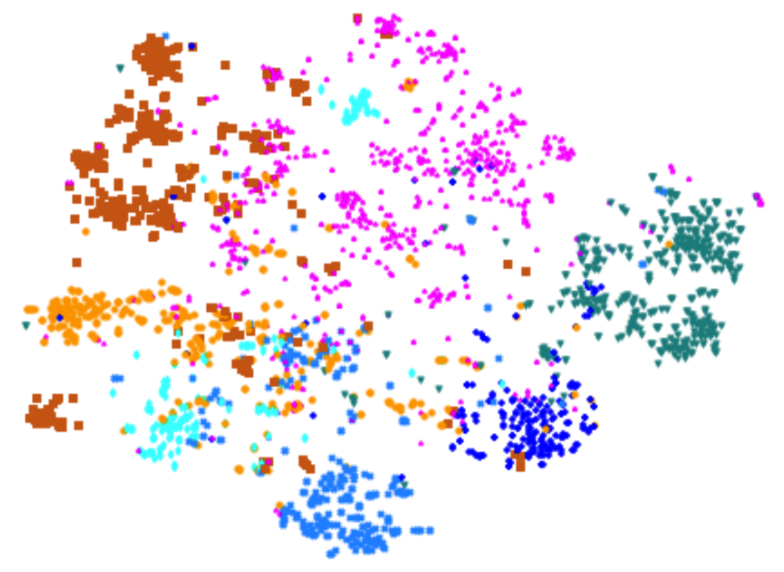
\includegraphics[width=0.6\textwidth]{./Figures/fig1.png}}
\end{center}
\label{fig:01}
\end{figure}

\end{frame}

%===========slide 1-4=======================
\section{Conclusions}
\begin{frame}{Conclusions}
\begin{itemize}
\setbeamertemplate{items}[ball]
\item Conclusions1.
\item Conclusions2.
\item Conclusions3.
\end{itemize}

\end{frame}


% ----------------------------------------------------------------------------
\begin{frame}
\ \\ \ \\
\centering {\Huge \textcolor{darkred}{\bf Thank You}}\\

\end{frame}

 
\end{document}